\section{Measurement of Capacitors}
The measurement of capacitor values are done as separate task by measurement of load time
after all other measurements. 
The original software of Markus F. did this with a program loop, which reads the corresponding digital input
pin until a switch occured and count the loop cycles.
This has the handicap, that the resolution of time measurement is limited by the
time consumption of one loop cycle.
This usually was done in all six combinations for all three probe pins. 
The actual software uses two different ways to get the load time in only
three combinations for the three probe pins. The positive side is now always the
higher probe number. Only if capacity is measured parallel with a diode, the
polarity can be in the other order.

\subsection{Discharging of Capacitors}
You should always discharge the capacitor before connecting it to the tester.
The tester additionally discharge the capacitor before any measurement.
If the voltage is below \(1300mV\), the capacitor is shortened by the output pins of the connected ADC port (Port C).
I~believe that this is legal because every output port has a built in resistance of about \(20\Omega\).
The data sheet Figure 149 (page 258) \cite{ATmega8} shows voltage drop of output pins up to \(2V\).
Of course I can not guaranty, that no damage can occur. 
I~have tested the function with big capacitors of more than \(15mF\) many times and I~have never noticed any problem.
The current should be below the specified limit of \(40mA\) and is reduced fast by discharging.
Off course damage can occur if you do not discharge a (high voltage) capacitor before connecting it to your tester.

\subsection{Measurement of big Capacitors}
\label{sec:bigcap}
One side of the capacitor is connected to GND. The other side of the capacitor is connected with the
\(680\Omega\) resistor to VCC for a period of 10ms. Afterwards this probe pin is switched to Input (High Impedance).
After this \(10ms\) current pulse the voltage of the capacitor is measured without any current. If the voltage has not
reached a minimal value of \(300mV\), the load pulse is repeated up to 499 times.
If after 127 pulses a minimum voltage of \(75mV\) is not reached (about 2s), further load is stopped, because never
the \(300mV\) can be reached with the remaining load pulses.
Figure~\ref{fig:bigcap} shows the three phases of measuring the capacity value of a capacitor.
The value of the capacity is then computed with the count of load pulses and the reached load voltage from a table.
The table contains  the factors to get the capacity in nF units from load time and the reached voltage
with a spacing of \(25mV\).
Interim value of voltage will be interpolated.

\begin{figure}[H]
\centering
 \begin{overpic}[width=.93\textwidth]{../FIG/Bigcap.pdf}
  \color{black}
  \put(25,97){\makebox(0,0)[cb]{Quick Discharge of capacitor}}
  \put(25,61){\makebox(0,0)[cb]{10ms Charge Phase of capacitor}}
  \put(25,26){\makebox(0,0)[cb]{Voltage Measurement Phase of capacitor}}
 \end{overpic}
\caption{discharge a capacitor and load with \(10ms\) load pulses until voltage reach a value of \(300mV\)}
\label{fig:bigcap}
\end{figure}
As a result of the low load voltage, the measurement is much faster than the initial software version,
 because this advantage works also on discharging. So bigger capacitors can be measured.
Furthermore a diode, which is parallel connected to the capacitor don´t disturb the measurement in most cases,
because the flux voltage of most diodes is not reached.
Beginning with software version 1.12k a trickery is used to measure the residual voltage of a capacitor
before the capacity measurement. 
Depending on the previous history of the capacitor the residual voltage can be positive or negative.
Negative voltages can not be measured with the ADC. For that reason the voltage of the negative test pin
is raised with the \(680\Omega\) resistor to about \(132mV\) as shown in figure~\ref{fig:CapResidV}.
With the difference of the voltages measured at both sides of the capacitor the residual voltage can
be build with any polarity. The voltage of the positive test pin remains positive in any case, even if
the capacitor have a negative residual voltage of some mV.

\begin{figure}[H]
\centering
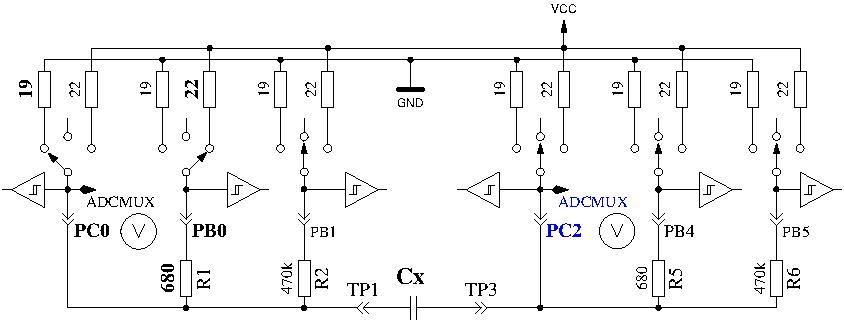
\includegraphics[width=.8\textwidth]{../FIG/Cap_residV.pdf}
\caption{Measurement of the residual voltage of a capacitor before loading}
\label{fig:CapResidV}
\end{figure}

Figure~\ref{pic:c229} shows the charge and discharge for a \(229\mu F\) capacitor.
The flat top of diagram from load end to discharge begin is caused by the measuring and computing time of the ATmega.
Figure~\ref{pic:c5mF} shows the same measurement for a~\(5mF\) capacitor,
notice how the time for measurement is grown to about 1.5 seconds inclusive the discharge. 
The last example shows the capacity measuring of a~\(15mF\) capacitor in Figure~\ref{pic:c15mF}

\begin{figure}[H]
  \begin{subfigure}[b]{.5\textwidth}
    \centering
    \includegraphics[width=1.\textwidth]{../PNG/charge_229uF.png}
    \caption{\(229\mu F\) Capacitor}
    \label{pic:c229}
  \end{subfigure}
  ~
  \begin{subfigure}[b]{.5\textwidth}
    \centering
    \includegraphics[width=1.\textwidth]{../PNG/charge_5mF.png}
    \caption{\(5mF\) Capacitor}
    \label{pic:c5mF}
  \end{subfigure}
  \caption{Charge and discharge of big Capacitors for measuring}
\end{figure}

\begin{figure}[H]
  \centering
    \includegraphics[width=.8\textwidth]{../PNG/charge_15mF.png}
  \caption{Charge and discharge of a \(15mF\) Capacitor for measuring}
  \label{pic:c15mF}
\end{figure}

After this capacity measurement the self-discharge of the capacitor will be checked by
waiting a proportional period the loading has taken and reading the load voltage again.
The measured capacity value is corrected due to this voltage drop.
A test with a parallel connection of a \(68\mu F\) capacitor and a \(2.2k\Omega\) resistor shows
the effectivity of this method.
The measured capacity value without the resistor is \(66.5\mu F\),
with the parallel \(2.2k\Omega\) resistor results to a capacity value of \(66.3\mu F\).
For comparison here are the results measured with a Peaktech 3315 multimeter:
Without the resistor a capacity value of \(68.2\mu F\) is measured, with the
parallel \(2.2k\Omega\) resistor a value of \(192\mu F\) is measured with the multimeter.


\subsection{Measurement of small Capacitors}
If the first \(10ms\) load pulse has overloaded the capacitor, another technique of measurement is used.
The ATmega processor has a build in 16-Bit counter, which can operate at the full clock rate (\(1MHz\) or \(8MHz\)).
This counter has also the feature to save his counter value by a external event.
This event can be built by the output of the comparator. 
The comparator can operate with any ADC input pin and the band gap reference.
Figure~\ref{fig:comparat} shows a simplified diagram of the measurement situation.
So I discharge the capacitor, prepare the comparator to the proper pin input, start the counter at 0 and
start immediately the charging of the capacitor with one side connected to GND and the other side connected with
the \(470k\Omega\) resistor to VCC.
Now I check within a program loop, if the counter flags signals a overflow event or a input capture (external) event.
I count the overflow events until I detect the input capture event.
In this case I stop the counter and check if I must count a additional overflow,
because the counter can't be stopped by the input capture event.


The input capture counter and the overflow counter built together the total time,
from which we can get the capacity with a factor.
The actual software can use a table with the theoretical  dependency of the load time in respect to the comparator voltage.
The table is spaced in \(50mV\) steps and will be interpolated according to the actual reference voltage. 
This table will only be acticated with the Makefile option WITH\_AUTO\_REF.
From the build capacity value I subtract a predefined experimental find out constant or a value found by the last selftest
with AUTO\_CAL option to eliminate the zero offset. 
The zero offset may vary with printed board type, the used test equipment or processor.
The selftest with AUTO\_CAL option will find out your zero offset automatically.

I noticed that the reference voltage is permanently somewhat to low,
 so that you can choose an offset with the Makefile option REF\_C\_KORR.
After calibration with the AUTO\_CAL option , the REF\_C\_KORR will only be a offset to the measured difference voltage
between loaded capacitor and internal reference.
The measured reference voltage will then be corrected (added) by your value (mV units).
If option WITH\_AUTO\_REF is not used, the reference voltages of ATmega8, ATmega168 and ATmega328
are applied as noted in the data sheets~\cite{ATmega8}~\cite{ATmega168}. 
A sample measurement of this type is shown in figure~\ref{pic:c22uF}.
The measurement time for the \(22\mu F\) capacitor is above \(2.6s\) because the \(470k\Omega\) is
used for charging. But discharging is in this case much faster than charging.

\begin{figure}[H]
\centering
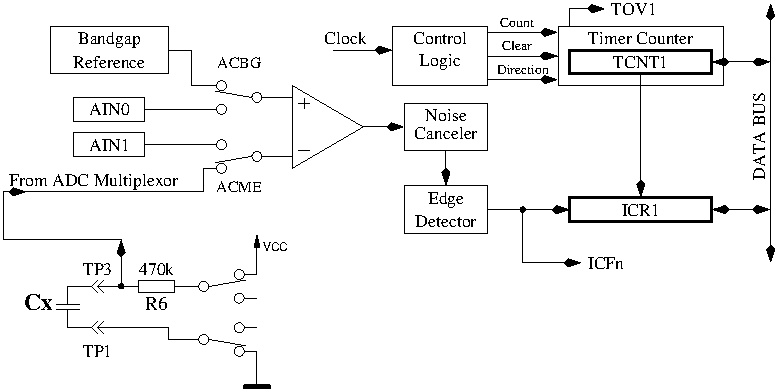
\includegraphics[width=.8\textwidth]{../FIG/Comparat.pdf}
\caption{measurement little capacity values with comparator}
\label{fig:comparat}
\end{figure}

\begin{figure}[H]
  \centering
    \includegraphics[width=.8\textwidth]{../PNG/charge_22uF.png}
  \caption{Charge and discharge of a \(22\mu F\) Capacitor for measuring}
  \label{pic:c22uF}
\end{figure}


In principle this technique of measurement can also be done with the \(680\Omega\) resistor, but 
because the ADC can't be used if the comparator is working, I have no chance to monitor the
load voltage until the comparator is stopped. If a undetected diode is parallel connected with
the capacitor, the load current of the capacitor can be absorbed by the diode (threshold voltage) and
the band-gap voltage will never be reached.
The method taken in actual software for big capacitors in section~\ref{sec:bigcap}
avoids this conceptual bug.

\subsection{Measurement of very small capacity values with the sampling technique}
The radio amateur Pieter-Tjerk (PA3FWM) has integrated the measurement capability for very small
capacity values (\textless~100pF) with the sampling technique.
The conversion period of the ADC is in fact too long for sampling a fast signal directly.
But the voltage of the input signal is hold at a specified time of the conversion cycle,
the Sample and Hold (SH) time.
The ADC need 13 clock cycles for a total conversion and the ADC clock is build by dividing the
processor clock by 128 or 64.
The input voltage is fixed at exactly ADC clock number 1.5 for continuous cycles.
If the input signal can be generated again and again, we can shift the sample time of the ADC from
one to the next signal repetition, so that we get a sample sequence of the fast signal.
A normal ADC cycle takes 13x64 = 832 clock cycles with a 8~MHz processor clock.
If we repeat the input signal with a 831 clock cycle, a uninterrupted ADC (free rum mode) would
sample the signal one processor clock tick later for every following signal repetition.
We must make sure with this method, that the first ADC sampling of the signal is done at
the requested starting time. The time of the following ADC samples would be shifted by one processor clock
tic later for every next signal repetition.
If the signal can be repeated exactly, the combined signal of many periods is the same, 
which would be sampled and converted directly with a ADC running with the processor clock (8~MHz).
Figure~\ref{fig:sampling} shows the principle of sampling a ten times repeated signal
to get 10 samples (SH0 - SH9).
In reality the relativ time shift of successive samples is much smaller than shown here.

\begin{figure}[H]
\centering
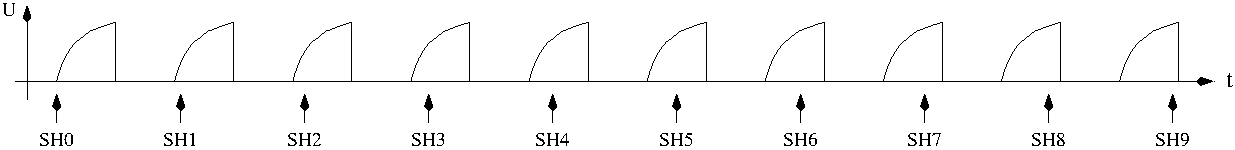
\includegraphics[width=1.\textwidth]{../FIG/sampling.pdf}
\caption{Scanning of a voltage curve with the sampling technique}
\label{fig:sampling}
\end{figure}

One problem to fix the exactly time of the first sample is given by a continuous running clock precaler.
Only a trigger of a external signal can reset the ADC clock divider.
The clock divider would resume with dividing, if the ADC is started by program intruction.
Only a program written in assembly language can specify the exactly points in time for
this sampling technique. Every clock tick is important for building the program loops.

By analysing the voltage characteristic of charging a small capacitor you can see, that the time constant
is not continuous during the sampling period. This was shown by Pieter-Tjerk at a presentation at
the ''60. UKW-Tagung in Weinheim''. The internal capacitor of about 10~pF, which hold the input voltage
for the conversion, is uncoupled at the SH time and connected again two ADC clock cycles later. 
Additionally there is a little jamming in the data just a half clock before the reconnection,
which is probably caused by the switch of the multiplexor.
Both disturbancies are respected with the data processing in the software.
The sampling software can handle up to 255 samples. The software can also build the mean value of
up to 32 charge sequencies. By building the mean value the effect of noise trouble will be less.
The sampling software can monitor and process both, the charge or the discharge of a capacitor.
Because both charge directions are used to measure the capacity value of a diode in reverse direction,
the calibration task measure the zero capacity value in both charge direction for all pin combinations.
By measuring the capacity value of a diode in both charge directions, the difference between both
values can be shown.
With the charge direction a capacity value is measured near the voltage 0 and with
the discharge direction the capacity is measured near a voltage of 5V.
With normal capacitors there is no difference in the capacity values with this little voltage difference detectable.
Therefore only the charge direction is used for measuring little capacities (\textless 100pF).

Pieter-Tjerk has optimized his function for a 16~MHz operation.
In this configuration you will get a resolution of 0.01~pF.
For the 8~MHz operation the ADC will run at the half speed for getting the above-mentiored disturbances
at the same data points compared to the 16-MHz operation.
The loss of resolution with the 8~MHz operation will be irrelevant for most users and the
additional testing time with the slower ADC in this mode is tolerable too.



\subsection{Measurement of the Equivalent Series Resistance ESR}
The series resistance ESR \cite{ESR} is a good indicator for the aging of electrolytical capacitors for example.
The figure ~\ref{fig:Cap_equiv} shows a equivalent circuit of a capacitor.
The resistor \(Rp\) represents the leakage resistance of the capacitor, \(ESL\) the equivalent series inductivity and
the resistance \(ESR\) represents the equivalent series resistance.

\begin{figure}[H]
  \centering
    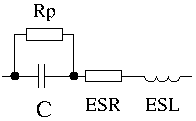
\includegraphics[width=.3\textwidth]{../FIG/Cap_equiv.pdf}
  \caption{Equivalent circuit of a capacitor}
  \label{fig:Cap_equiv}
\end{figure}

Usually the data sheets publish ESR values, which are measured with a frequency of 100 kHz and a temperture 
of 20\textdegree C .
The figures \ref{fig:Cap_FC_data} and \ref{fig:Cap_FR_data} shows the ESR values of the Panasonic series FC and 
the ''low ESR'' series FR.
Both series are able to operate up to a temperature of 105\textdegree C.
The figure \ref{fig:Cap_FC_FR_data} shows the data of both series with a allowable working stress of \(25V\).
If the series have different types with the same capacity and voltage range, the one with the lowest ESR is
taken for the diagram.
The values of capacity and ESR of electrolytic capacitors change significant with there operating temperature.

\begin{figure}[H]
  \centering
    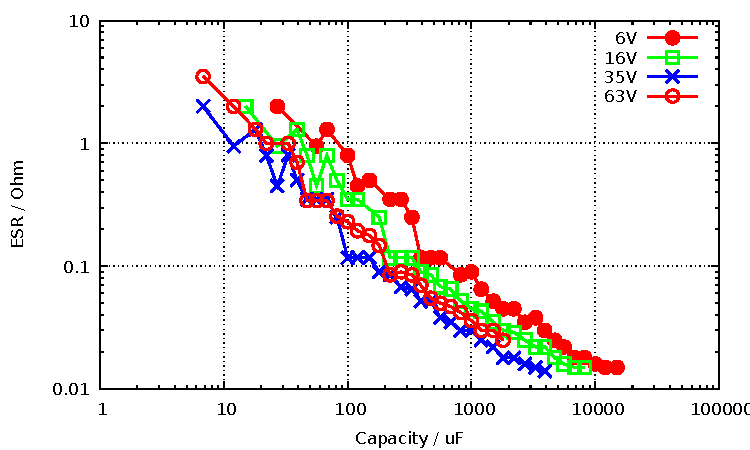
\includegraphics[width=.8\textwidth]{../GNU/Cap_FC_data.pdf}
  \caption{ESR data from the Panasonic data sheet of the series FC}
  \label{fig:Cap_FC_data}
\end{figure}

\begin{figure}[H]
  \centering
    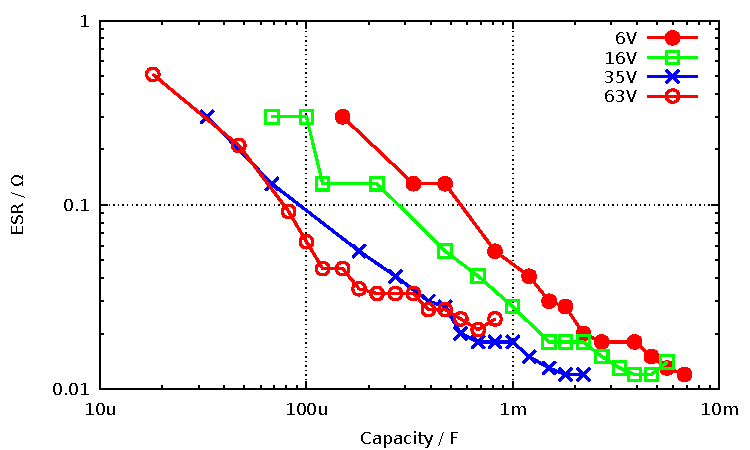
\includegraphics[width=.8\textwidth]{../GNU/Cap_FR_data.pdf}
  \caption{ESR data from the Panasonic data sheet of the series FR}
  \label{fig:Cap_FR_data}
\end{figure}

\begin{figure}[H]
  \centering
    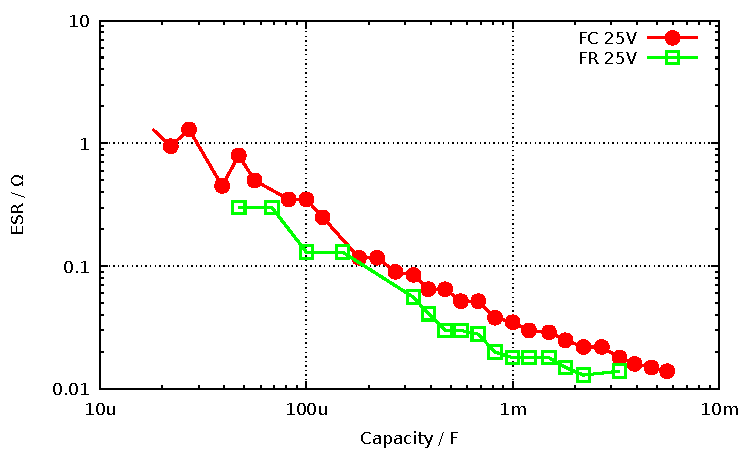
\includegraphics[width=.8\textwidth]{../GNU/Cap_FC_FR_data.pdf}
  \caption{Comparison of the ESR data from series FC with series FR}
  \label{fig:Cap_FC_FR_data}
\end{figure}

There is no simple way to measure the ESR with a frequency of 100 kHz with the ATmega hardware,
because neither the ADC can sample a so high input frequency, nor the existing circuit can support
with a \(100kHz\) signal.
At next there will be introduced two method's for the measurement of the ESR, which both manage on 
the existing circuit.
Both method's use a rectangular signal for the measurement, so that the results will never be
the same with the values measured with sinusoidal signal.
With the first method the measured values are close to those values, which are measured with a
\(1kHz\) signal. 
But the second method has the advantage, that the zero value can be determined with shorted test pads and
that additionally the measured ESR is more close to the value measured with \(10kHz\) signal.
Currently I have no idea for a measurement method, which can produce a ESR value close to the
value of a \(100kHz\) measurement.

The following table \ref{tab:capESR} should show the dependency of the ESR results from measurement frequency.
All capacitors without the \(47\mu F\) capacitor are from the same FC series of manufactor Panasonic.
The reference values are measured with a Peaktech 2170 LCR meter.
All results of the TransistorTester are measured with the method 2 of subchapter \ref{sec:ESR2} .
Capacitors with big capacity values are difficult to measure with higher frequencies like \(100kHz\) because
the inductance ESL make trouble.

\begin{table}[H]
  \begin{center}
    \begin{tabular}{| l | c | c | c | c | c |}
   \hline
            & Data sheet & PeakTech  & Peaktech & PeakTech & Transistor- \\
Capacitor   & 100~kHz    & 100~kHz   & 10~kHz   & 1~kHz    & tester  \\
    \hline
    \hline
1uF / 50V    & 2.4       & 1.27      & 1.75     & 4.31     &  2.1 \\
    \hline
2.2uF / 50V  & 1.8       & 1.07      & 1.34     & 2.76     &  1.6 \\
    \hline
4.7uF / 50V  & 1.3       & 1.19      & 1.40     & 2.37     &  1.5 \\
    \hline
4.7uF / 50V  & 1.3       & 1.19      & 1.40     & 2.37     &  1.5 \\
    \hline
10uF / 50V   & 1.3       & 1.26      & 1.45     & 2.05     &  1.5 \\
    \hline
22uF / 10V   & 2.0       & 1.52      & 1.76     & 2.24     &  1.9 \\
    \hline
47uF / 63V   & ?         & 0.46      & 0.50     & 0.63     &  0.52 \\
    \hline
    \end{tabular}
  \end{center}
  \caption{ESR values of different electrolytical capacitors}
  \label{tab:capESR} 
\end{table}


\subsection{Measurement of the Equivalent Series Resistance ESR, first way}
If the measured capacitor has a capacity of more than \(0.45\mu F\), the tester will try to measure
the series resistance too.
For a capacity of more than \(3.6\mu F\) the normal clock rate of \(125kHz\) for the Analog-Digital converter is used.
For lower capacities the higher clock rate of \(500kHz\) is used to accelerate the measurement.
The accuracy of the ADC results will be more worth by the higher clock rate, but this could be accepted by the
higher ESR values of capacitors with lower capacity.
Otherwise the measurement of ESR with this method is not possible for a capacity of less than \(1.8\mu F\) at the normal
clock rate of \(125kHz\).

Strictly speaking the ESR of a capacitor depends on the operating frequency and temperature.
Usually the value measured with sine wave-form signal of \(100kHz\) is denoted in the data sheets.
This measurement can not be done with the ATmega without external equipment.
With the subsequent written method the measurement frequency with the standard ADC clock rate will be below 640 Hz
with nearly rectangular signal. With \(500kHz\) ADC clock rate the measurement frequency will be 2400 Hz.
To get the value of the equivalent series resistance,
the voltage of both connections will be measured during loading in one direction with the ADC internal reference 
voltage (\(1.1V\)).
After the measurement the load current will be switched off and the voltage of the capacitor is measured
again without the current.
If this voltage is below \(3mV\), the sequence of measurement is repeated.
The figure~\ref{fig:Cap_esr} shows the corresponding circuits.

\begin{figure}[H]
 \centering
  \begin{overpic}[width=.83\textwidth]{../FIG/Cap_esr.pdf}
   \color{black}
   \put(28,85){\makebox(0,0)[cb]{Voltage measurement with charge current}}
   \put(28,40){\makebox(0,0)[cb]{Voltage measurement without current}}
  \end{overpic}
 \caption{Circuit of the ESR measurements of a capacitor}
 \label{fig:Cap_esr}
\end{figure}

The difference of capacitor voltages with and without current is proportional to the internal resistance of the capacitor. 
The expected voltage of this difference is so low, that one measurement can not result to a feasible result.
Therefore after this the current will be switched to the opposite direction and the same measurement will be repeated.
The whole measurement sequence will be done 128 times and the results of the voltage measurements will be added.
So we have three sums of voltages, the voltage \(Ulp\) at the low side of the capacitor with current, the voltage \(Uhp\) at
the high side of the capacitor with current and the voltage \(Uc\) of the high side of the capacitor without current.
The sum of voltages at the low side of the capacitor represents the potential drop with the mean load current at
the port output resistance \(Rport\). 
The voltage difference  of the high side and the low side of the capacitor represents the voltage of the capacitor with
load current \(Udiff = Uhp - Ulp\).
The difference \(Uesr = Udiff - Uc\) should represent the voltage drop at the internal resistance of the capacitor with
mean load current.
We will get the resistance value with the relation of this voltage \(Uesr\) to the voltage \(Ulp\), scaled with the
known resistance value of the port output \(Rport\).
The scale factor is selected to get a resistance resolution of \(0.01\Omega\):  \(Resr = \frac{Uesr \cdot 10 \cdot Rport}{Ulp}\)
The figure~\ref{pic:esr4} shows a part of the voltage curve of a \(4.2\mu F\) capacitor during the ESR measurement.
To explain the influence of the ESR, a series \(6.8\Omega\) resistor is added to the capacitor.
The little voltage break after loading the capacitor is interpreted by software to get the ESR.
The greater voltage drop of the measurement to GND potential is caused by the port output resistance of about \(20\Omega\).
For this measurement a total ESR of \(7.5\Omega\) is reported by the tester, without the series \(6.8\Omega\) resistor a ESR of \(0.56\Omega\) is found.
The figure~\ref{pic:esr2} shows the same measurement with higher measurement frequency of a \(2.2\mu F\) electrolytical capacitor
with a ESR of \(6.5\Omega\).


\begin{figure}[H]
  \begin{subfigure}[b]{.5\textwidth}
    \centering
    \includegraphics[width=1.\textwidth]{../PNG/ESR_4uF.png}
    \caption{measured one pin to GND}
  \end{subfigure}
  ~
  \begin{subfigure}[b]{.5\textwidth}
    \centering
    \includegraphics[width=1.\textwidth]{../PNG/ESR4uF6R8.png}
    \caption{measured pin to pin}
  \end{subfigure}
  \caption{Voltage curve of a \(4.2\mu F\) capacitor during the ESR measurement}
  \label{pic:esr4}
\end{figure}


\begin{figure}[H]
  \begin{subfigure}[b]{.5\textwidth}
    \centering
    \includegraphics[width=1.\textwidth]{../PNG/ESR_2uF_pin2GND.png}
    \caption{measured one pin to GND}
  \end{subfigure}
  ~ 
  \begin{subfigure}[b]{.5\textwidth}
    \centering
    \includegraphics[width=1.\textwidth]{../PNG/ESR_2uF_pin2pin.png}
    \caption{measured pin to pin}
  \end{subfigure}
  \caption{Voltage curve of a \(2.2\mu F\) capacitor during the ESR measurement}
  \label{pic:esr2}
\end{figure}



The accuracy of the ESR measurement is not very high by different reasons:
\begin{enumerate}
\item The voltage measurement at both pins of the capacitor can not be done at the same time, the only way is to do it in sequence.
In the interim time between both measurements the load current has changed due to the charge of capacitor.
The program tries to compensate this fact with a capacity dependent correction of the low side voltage.
\item The ADC takes the measurement voltage after 1.5 clock ticks after the start of conversion.
The conversion beginns with the rising edge of the ADC-clock, if the start bit is set.
If the charge current will be switched off to early, the ADC takes the wrong voltage for the measurement with current.
If the charge current will be switched off to late, the capacitor will take more electric charge, than that of the
corresponding measurement with load current. This will cause a too high voltage of the measurement without current.
But it is difficult to switch off the current at the right time by software. 
\item The port output resistance is used as a reference value by this measurement method, but this resistance value is
not exacly known too.
\item The resolution of the ADC is not sufficient to get a resolution of resistance of \(0.01\Omega\).
To get the best avaiable resolution of ADC, the internal reference (\(1.1V\)) is used for all measurements.
The resolution deficit will be attenuated by accumulating a big number of single measurements too.
\item The switching of ports can not be exactly synchronized to the ADC clock with polling of conversion done.
\end{enumerate}

Anyway the results seems to be practical, as shown with the following figure \ref{fig:Cesr}.
The ESR values of the same part measured with the Transistortester vary more than the values measured with the LCR meter.
The ESR values from the LCR meter are measured with a frequency of \(1kHz\) or are interpolated for little capacities to
\(2.4kHz\).
You must respect the quality of all connection parts. The used cable connections can cause a higher measured resistance value.
The plug connectors can also result a higher resistance value.
The LCR meter has the advantage of the used Kelvin terminals.
Only one capacitor with a capacity below \(1\mu F\) was a \(500nF\) ceramic type, all others were
plastic film capacitors.
The only electrolytical capacitor of the test series below \(9\mu F\) was a \(2.2\mu F\) capacitor.

\begin{figure}[H]
\centering
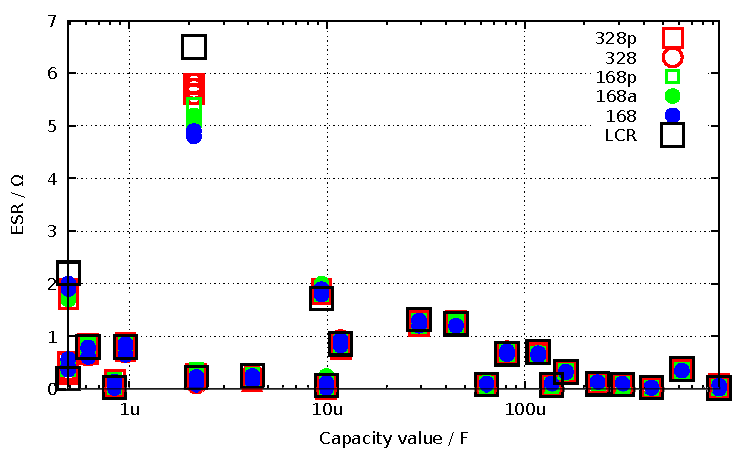
\includegraphics[width=.93\textwidth]{../GNU/Cesr.pdf}
\caption{ESR measurement results of 15 different ATmega}
\label{fig:Cesr}
\end{figure}


\subsection{Measurement of the Equivalent Series Resistance ESR, second way}
\label{sec:ESR2}
From beginning with software version 1.07k the ESR measurement way is changed to a new measurement method.
The different measurement steps are shown in figure~\ref{fig:Cap_esr2}. The difference to the previous way is that
the period of current flow through the capacitor is essential shorter.
The capacitor is preloaded with a half pulse to the negative direction and is than loaded in a cyclic way in both
direction.
The timing of the load pulse is so selected, that the middle of the load puls at sample 4 and 8 is
pointed to the sample and hold time of the ADC (2.5 clock tics after start of ADC). 
A complete measurement cycle is shown in figure~\ref{fig:Cap_esr2_timing}.
The sums of 255 measurement cycle results is used for getting a result with adequate resolution. 
A continuing charge of the capacitor in any direction is avoided by the same charge and discharge pulse length
and the same circuit.
By measuring the reference voltage the capacitor remains currentless. By that this measurement are not time critital.
It is only assumed, that the capacitor hold the voltage until the next charge or discharge pulse begins.

\begin{figure}[H]
  \centering
    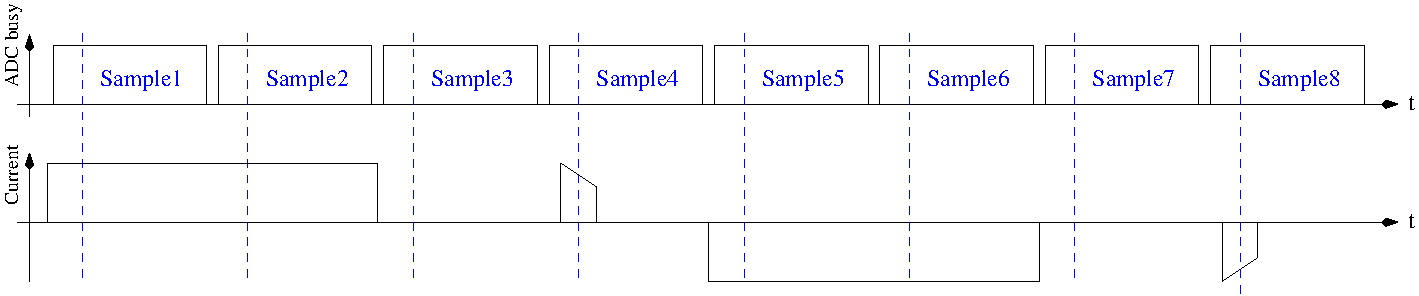
\includegraphics[width=1.\textwidth]{../FIG/Cap_esr2_timing.pdf}
  \caption{Timing of a measurement cycle for the new ESR-measurement way}
  \label{fig:Cap_esr2_timing}
\end{figure}

\begin{figure}[H]
 \centering
  \begin{overpic}[width=.83\textwidth]{../FIG/Cap_esr2.pdf}
   \color{black}
   \put(20,98){\makebox(0,0)[cb]{Forward reference measurement}}
   \put(20,72){\makebox(0,0)[cb]{Forward voltage measurement with probe current}}
   \put(20,47){\makebox(0,0)[cb]{Reverse reference measurement}}
   \put(20,21){\makebox(0,0)[cb]{Reverse voltage measurement with probe current}}
  \end{overpic}
 \caption{More simple ESR measurement of a capacitor}
 \label{fig:Cap_esr2}
\end{figure}


Due to the shorter load puls not only the ESR of capacitors with lower capacity can be measured, but this
way of measurement can also be used for the measurement of resistors with little resistance, if they don't
have a detectable inductance. By doing that, a resolution of \(0.01\Omega\) for this resistors can be achieved.
Also the zero resistance can be detected by the calibration part of the selftest for all three test pin combination.
You should keep in mind, that stable plug sockets or clamping connectors are essential for stable results.
The measurement periode is about \(900\mu s\), which results to a frequency of about \(1.1kHz\).
Because the load pulse is very short, the measurement result is comparable to measurements with \(10kHz\).
A measurement example with a \(10\mu F\) foil capacitor, once measured alone and once measures with a \(2.7\Omega\)
series resistor is shown in figure~\ref{pic:NewEsr10}.
You can see the effect of the additional resistance by comparing both diagrams.
You can see also, why the ADC measurement (SH) should point to the middle of the load pulse.
With big capacity values the load current is nearly stable during the total pulse length,
so you will get the middle voltage at the middle time of the load pulse. 
With lower capacity values you will get a significant difference, which can be compensated by the
known capacity value.

\begin{figure}[H]
  \begin{subfigure}[b]{.5\textwidth}
    \centering
    \includegraphics[width=1.\textwidth]{../PNG/NewEsr10uF0R0.png}
    \caption{without series resistance}
  \end{subfigure}
  ~
  \begin{subfigure}[b]{.5\textwidth}
    \centering
    \includegraphics[width=1.\textwidth]{../PNG/NewEsr10uF2R7.png}
    \caption{with \(2.7\Omega\) series resistance}
  \end{subfigure}
  \caption{Voltage curve of a \(10\mu F\) capacitor during new ESR measurement}
  \label{pic:NewEsr10}
\end{figure}


By using the \(27\mu s\) long charge pulses the ESR of capacitors above \(180nF\) can be determined.
For measuring of capacitors with lower capacity the current pulse is shortened to \(8\mu s\) for version 1.11k.
The figures~\ref{pic:NewEsr2} show the voltage curve of a \(2.2\mu F\) capacitor without and with
a \(2.7\Omega\) series resistor.

\begin{figure}[H]
  \begin{subfigure}[b]{.5\textwidth}
    \centering
    \includegraphics[width=1.\textwidth]{../PNG/NewEsr2u2F0R0.png}
    \caption{without series resistance}
  \end{subfigure}
  ~
  \begin{subfigure}[b]{.5\textwidth}
    \centering
    \includegraphics[width=1.\textwidth]{../PNG/NewEsr2u2F2R7.png}
    \caption{with \(2.7\Omega\) series resistance}
  \end{subfigure}
  \caption{Voltage curve of a \(2.2\mu F\) capacitor during new ESR~measurement with \(8\mu s\) charge pulses}
  \label{pic:NewEsr2}
\end{figure}

Because you can not see the sample and hold time of the ADC in the figures \ref{pic:NewEsr2},  the voltage curve is shown zoomed
in figures~\ref{pic:NewEsr2zoom}. The sample and hold time is approximately in the middle of the screen picture.

\begin{figure}[H]
  \begin{subfigure}[b]{.5\textwidth}
    \centering
    \includegraphics[width=1.\textwidth]{../PNG/NewEsr2u2F0R0zoom.png}
    \caption{without series resistance}
  \end{subfigure}
  ~
  \begin{subfigure}[b]{.5\textwidth}
    \centering
    \includegraphics[width=1.\textwidth]{../PNG/NewEsr2u2F2R7zoom.png}
    \caption{with \(2.7\Omega\) series resistance}
  \end{subfigure}
  \caption{Zoomed voltage curve of a \(2.2\mu F\) capacitor during new ESR~measurement with \(8\mu s\) charge pulses}
  \label{pic:NewEsr2zoom}
\end{figure}
 

The measurement results of the new ESR measurement method is shown in figure~\ref{fig:Cesr2}.
The ESR values are different from the results shown for the previous mesurement procedure in figure~\ref{fig:Cesr} because 
the ESR is frequency dependence of the ESR.
The reference values are determined with a LCR meter at a measurement frequency of \(10kHz \).

\begin{figure}[H]
\centering
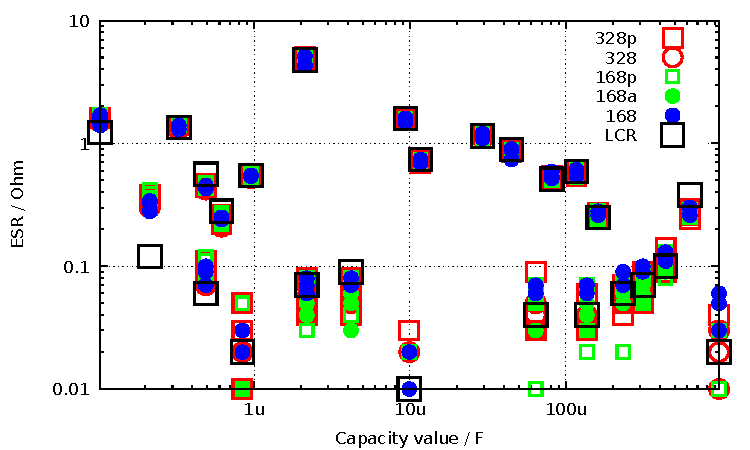
\includegraphics[width=.93\textwidth]{../GNU/Cesr2.pdf}
\caption{ESR results with 15 different ATmega, method 2}
\label{fig:Cesr2}
\end{figure}

A measurement series with different sized electrolytic capacitors are shown in figure \ref{fig:ElcoESR}.
The results of a PeakTech 3315 LCR meter of measurements with different frequencies and the results of the
TransistorTester are shown together. The resistance is illustrated with logarithmic scale in this diagram. 
In all cases the results of the TransistorTester is near by the results of
the \(10kHz\) measurements of the LCR meter.
Only the \(500\mu F/3V\) capacitor is a older exemplar, all others capacitors are as good as new.

\begin{figure}[H]
\centering
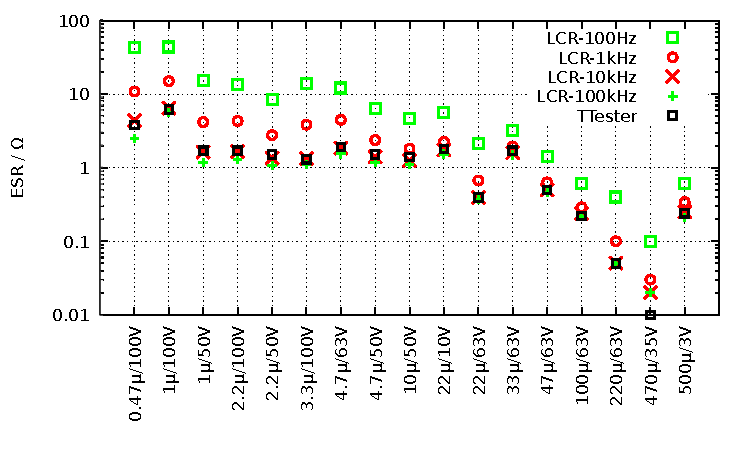
\includegraphics[width=1.\textwidth]{../GNU/Elco_esr.pdf}
\caption{Results of the ESR measurements of different electrolytic capacitors}
\label{fig:ElcoESR}
\end{figure}


Because the new measurement method can be taken for measuring of resistors with low values, the
measurement errors of some resistors below \(10\Omega\) with three example of each ATmega type will be shown in
figure~\ref{fig:res_esr}. 

\begin{figure}[H]
\centering
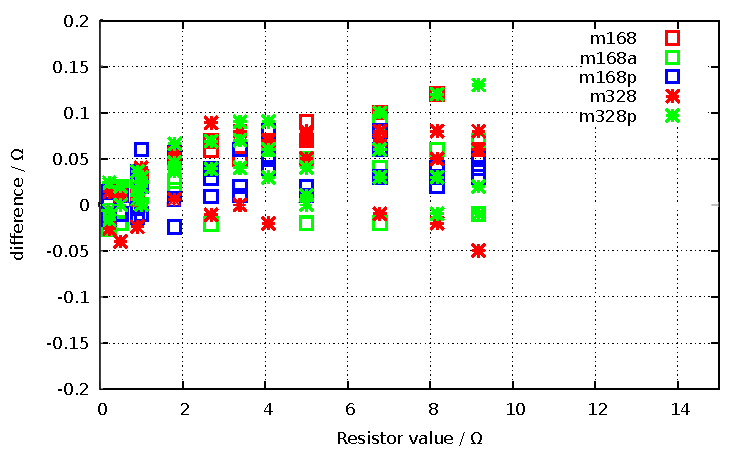
\includegraphics[width=1.\textwidth]{../GNU/res_esr.pdf}
\caption{Measurement errors of resistors with the ESR method}
\label{fig:res_esr}
\end{figure}

With software version 1.12k the load pulse length for the capacitors is reduced to \(2\mu s\) to accomplish ESR measurements
of capacitors with lower capacity values. Now a ESR-value can be measured for capacity values above \(20nF\).
But the measurement error will grow for lower capacity values. The reason for that is the decrease of the time constant of the
RC-circuit, which will be only about \(14.4\mu s\) for a capacity value of \(20nF\).
This will result to a fast change of the capacitor voltage during the \(2\mu s\) current pulses.
The software can select the sampling instance of the ADC only to the time of any processor clock.
But the input filter of the ADC has a time constant of about \(0.24\mu s\), which can vary from exemplar to examplar of the ATmega.
This change of the ADC input filter time constant can not be respected with the software.
For this purpose the ADC sample time must be selectable to a fraction of the processor clock period.
With greater capacity values of the measurement object the time constant will grow and the voltage change during the
load pulse will decrease. For this reason the variation of the ADC input filter time constant  has
lower effect with greater capacity values.
The examples in figures~\ref{pic:Cesr_22n} show the results for some capacitors with 10 different tester examples. The picture at the left side
shows the ESR results of some capacitors with higher ESR values. The result is rather simular compared with the results
of the Peaktech 2170 LCR meter at \(10kHz\) and at \(100kHz\).
At the right picture you can see the measurement results of some high quality capacitors with low ESR values.
Altough you can notice the limit of the method especially for low capacity values, the result is still better than no information.
In either case you can classify the quality of a capacitor also for lower capacity values.

\begin{figure}[H]
  \begin{subfigure}[b]{.5\textwidth}
    \centering
    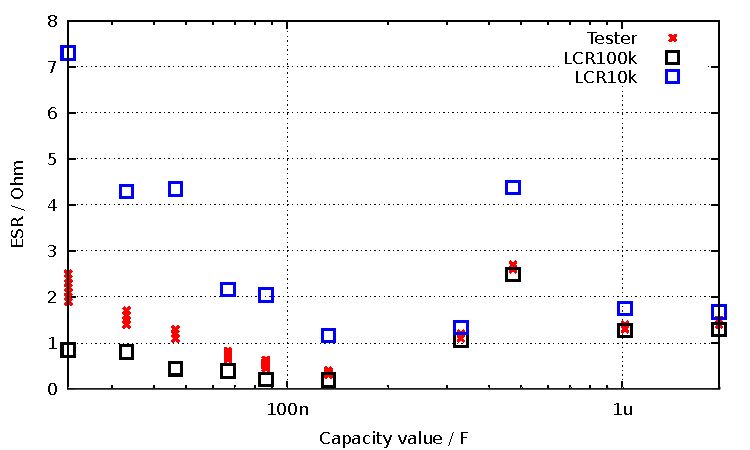
\includegraphics[width=1.\textwidth]{../GNU/Cesr_22n.pdf}
    \caption{higher ESR values}
  \end{subfigure}
  ~
  \begin{subfigure}[b]{.5\textwidth}
    \centering
    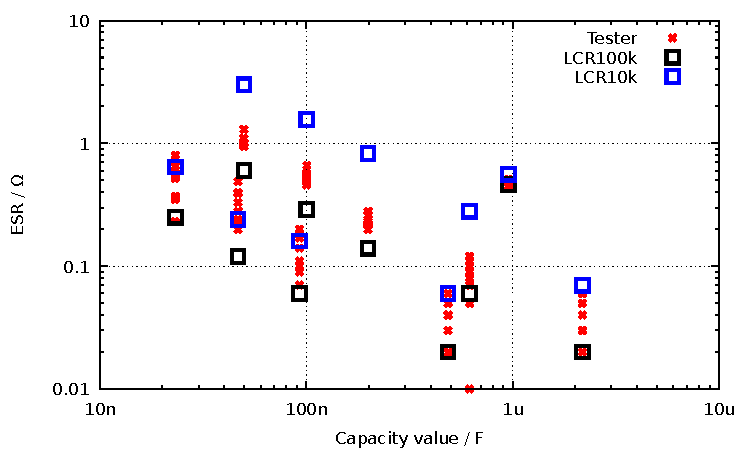
\includegraphics[width=1.\textwidth]{../GNU/Cesr_22n_low.pdf}
    \caption{lower ESR values}
  \end{subfigure}
  \caption{ESR-measurements of capacitors with lower capacity}
  \label{pic:Cesr_22n}
\end{figure}
 
For processors with more than 16K flash memory the \(470k\Omega\) resistor is connected parallel to the \(680\Omega\) resistor
for the half of single measurements beginning with software release 1.12k to vary the measurement current a little bit.
Unfortunately the additional current is very low, so that the resulting voltage enhancement can mot make shure a
change of the ADC result.
The voltage enhancement is only about 20\% of a ADC bit with the internal \(1.1V\) reference.
A add of a little noise voltage at the ADC input would be preferable.
With that feature a statistical enhancement of the ADC resolution by averaging can be achieved.
 


\subsection{Voltage loss after a load pulse, Vloss}
With the measurement of capacitors with big capacity values the voltage loss after the loading is analysed.
The reached load voltage is lost with electrolytic capacitors after a short periode.
This voltage loss can be caused by a parallel connected resistor.
But I assume, that this voltage loss of electrolytic capacitors is caused by a internal load dispersion directly
after the load pulse. By loading the capacitors with the \(470k\Omega\) resistor, as it is done for little
capacity values, this dispersion is already done after switching off the current.
No voltage loss is detectable for this case. But if you load the same capacitor with a short current pulse,
you can also detect the voltage loss for capacitors with lower capacity.
The same effect with lower loss can also be noticed for ceramic type capacitors. 
I have noticed, that capacitors with more than some \% voltage loss are suspect.
Especially noticable with respect to the voltage loss are older paper type capacitors, which are for other measurement
a problem too. Some measurement examples will be shown in the following table.
\vspace{0.5 cm}

\begin{tabular}{| l | c | c | c | c | c | c |}
   \hline
capacitor & Nenn-      & PeakTech      & Voltcraft & PeakTech & Transistor- \\
type        & capacity  & LCR 2170     & M2650-B   &  3315    & Tester      \\
    \hline
    \hline
paper     & 4700pF      & 6.75-10.36nF & 8.00nF    &  25.40nF & 10.71nF  \\
          &             & Q=2.5-32     &           &          & Vloss=11\% \\
    \hline
paper     & 6800pF      & 9.40-11.40nF & 10.41nF   &  23.30nF & 11.65nF \\
          &             & Q=5-25       &           &          & Vloss=5.0\% \\
    \hline
unknown  & 4700pF      & 5.85-6.33nF & 6.12nF    &  6.90nF  & 6225pF \\
           &             & Q=16-87     &           &          & Vloss=1.7\% \\
    \hline
foil      & 7870pF      & 7.86-7.87nF  & 7.95nF    &  7.95nF  & 7872pF \\
          &             & Q= \textgreater 1540     &           &          & Vloss=0\% \\
    \hline
paper     & 22000pF     & 37.4-57.5nF  & 52.8nF    &  112nF   & 118.5nF \\
          &             & Q=2.5-32     &           &          & Vloss=12\% \\
    \hline
foil      & 22600pF     & 22.4-22.5nF  & 22.57nF   & 22.69nF  & 22.54nF \\
          &             & Q= \textgreater 1540     &           &          & Vloss=0\% \\
    \hline
paper     & 100nF       & 144-256nF    & 177nF     &  318nF   & 529.7nF \\
          &             & Q=2.6-28     &           &          & Vloss=12\% \\
    \hline
ceramic   & 100nF       & 97.7-102nF   & 103.7nF   & 103.3nF  & 103.1nF \\
          &             & Q=90-134     &           &          & Vloss=0.1\% \\
    \hline
foil      & 100nF       & 98.0-101nF   & 101.4nF   & 102.2nF  & 101.6nF \\
          &             & Q=58-700     &           &          & Vloss=0\% \\
    \hline
\end{tabular}
\vspace{0.5 cm}

In this table you will find, that the capacity of all foil type capacitors can be measured by all intruments
with good precision.
The capacity values and the quality factor Q of the PeakTech LCR meter are minimum and maximum values of the
measurements in the frequency range \(100Hz\) to \(100kHz\).
At all examples in the table the voltage loss Vloss of the TransistorTester is big,
if the capacitors have a low quality factor.
Only in this case the differences of the capacity measurement results are also big.
The TransistorTester can only determine the voltage loss, if the measured capacity is more than \(5000pF\).

\subsection{Separate capacity and ESR measurement}
The separate capacity measurement and the afterwards measured ESR is only available for ATmega with sufficient 
memory with the handling dialog. This way of measurement is usefull for measurement of capacitors in the
circuit without desoldering.
Please take care, that all capacitors of the printed board are discharched before starting any measurement!
To realize the measurement in the soldered state, the measurement voltage is hold
to a low level of a little above \(300mV\) only.
In addition to that the measurement is only done with the \(680\Omega\) resistor to prevent a
big effect of connected components on the printed board.
To enable the measurement of capacitors with little capacity value, the first load puls is only
\(200\mu s\) short. If the loaded voltage let expect, that the \(300mV\) would not be reached with
a load pulse of \(2ms\), the next load pulse is done with \(2ms\) length.
When the capacity value of the measured capacitor is very high, the voltage grow is still low
with the \(2ms\) pulse. In this case the next load pulse(s) will be done with \(20ms\) length.
If the loaded Voltage grow near to \(300mV\), the shorter load pulses will be used again.
The total time of load pulses is added and after the load voltage has passed over \(300mV\), the
capacity value is computed from load time and the loaded voltage.
With this method capacity values of a little below \(2\mu F\) can be measured. The upper limit for the capacity
values is given with the restricted load time of \(2.5s\) to about \(50mF\).
If the capacity value is successfully measured, the ESR value of the capacitor is measured with the
method already described in section~\ref{sec:ESR2}.
The result is shown only short and then the next measurement is started immediately.
The series of mesurement is stopped after 250 measurements or after pressing the start key.
After finishing the measurements the program returns to the handling dialog.



\subsection{Results of Capacitor measurement}
The results of my capacity measurements are shown in figure~\ref{fig:mega8cap} for three ATmega8 processors.
Additionally some values of original software are shown with a correction factor of 0.88 (-12\%).
Other measurement results of different ATmega8 versions are shown in figure~\ref{fig:mega8Acap} and \ref{fig:mega8Lcap}.
The results of the measurement of the same capacitors for a ATmega168 is shown in figure~\ref{fig:mega168cap}.
The base for the error computing are the measurement results of a PeakTech 2170 RCL-meter, not the printed value
of the parts.
A part of the relative high measurement difference is caused by the too high measurement frequency of the RCL-meter for big
electrolytical capacitors. On the other side the bad quality factor of the electrolytical capacitors may cause
another percentage.

\begin{figure}[H]
\centering
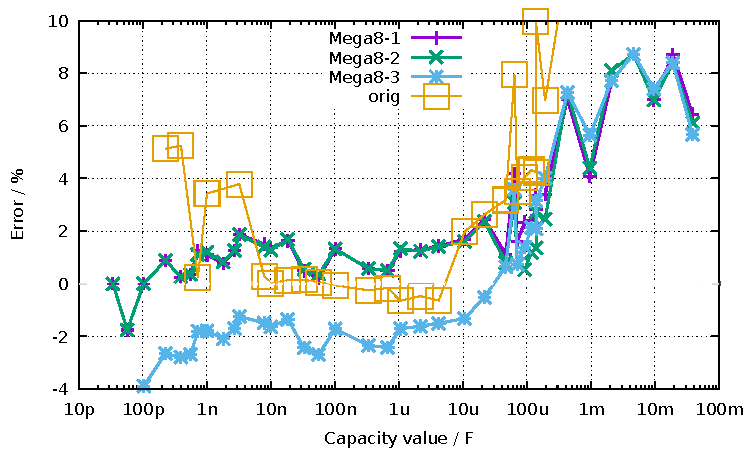
\includegraphics[width=1.\textwidth]{../GNU/Mega8cap.pdf}
\caption{Error in \% for capacitor measurements with ATmega8 }
\label{fig:mega8cap}
\end{figure}

\begin{figure}[H]
  \begin{subfigure}[b]{.5\textwidth}
    \centering
    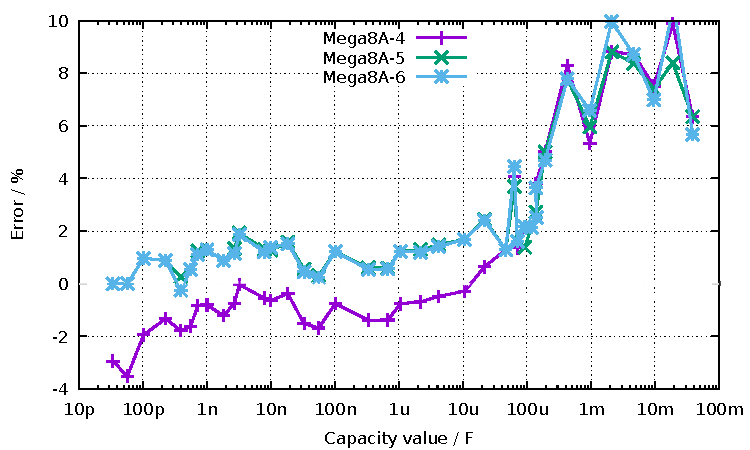
\includegraphics[width=1.\textwidth]{../GNU/Mega8Acap.pdf}
    \caption{with three ATmega8A}
    \label{fig:mega8Acap}
  \end{subfigure}
  ~
  \begin{subfigure}[b]{.5\textwidth}
    \centering
    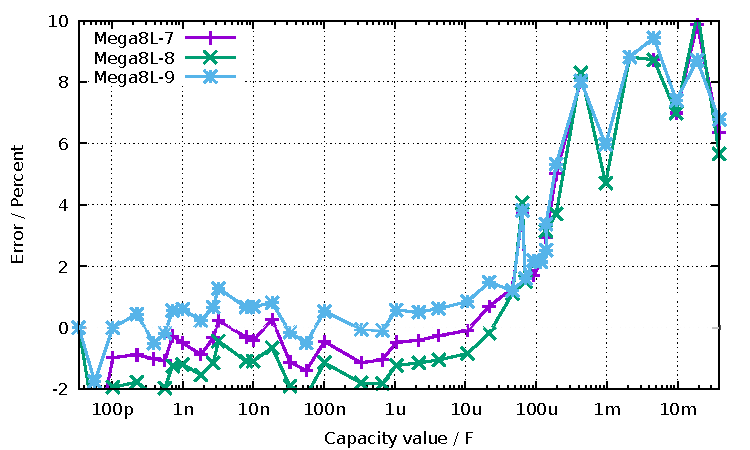
\includegraphics[width=1.\textwidth]{../GNU/Mega8Lcap.pdf}
    \caption{with three ATmega8L}
    \label{fig:mega8Lcap}
  \end{subfigure}
  \caption{Relative error of capacitor measurement}
\end{figure}

\begin{figure}[H]
\centering
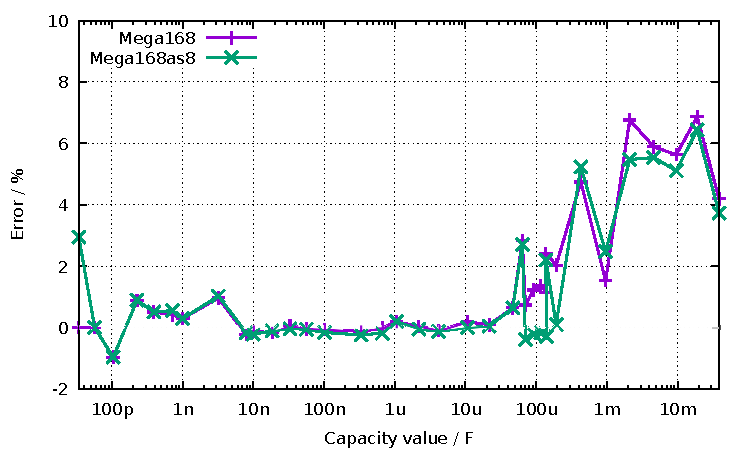
\includegraphics[width=1.\textwidth]{../GNU/Mega168cap.pdf}
\caption{Error in \% for capacitor measurements with ATmega168 }
\label{fig:mega168cap}
\end{figure}

Figure~\ref{fig:capcompare} illustrates, how difficult is it to choose the right base for the capacity measurement.
All measurement results are compared with the best estimated value of the capacitors.
The gradient ,,Multimeter'' shows the differences of the Peaktech~3315 Multimeter results.
The next gradient ,,LCR'' shows the differences of the Peaktech~2170 LCR-Meter results, which is taken from best frequency approach.
To compare this results to the results of a ATmega168 equipped Transistor-Tester the gradient ,,ATmega168as'' is also shown.
I beleave, that this errors are not real measurement errors of the particular equipment, because my best estimated value are
also not the real capacity value of the capacitors.

\begin{figure}[H]
\centering
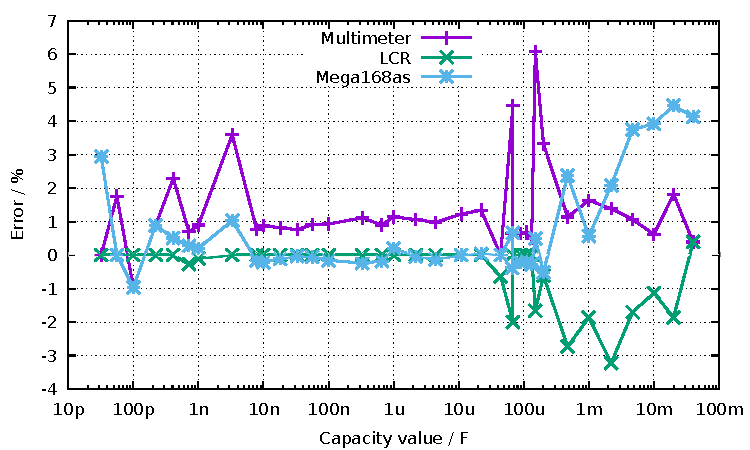
\includegraphics[width=1.\textwidth]{../GNU/capcompare.pdf}
\caption{Comparison of capacity measurement results of Multimeter, LCR-meter and ATmega168}
\label{fig:capcompare}
\end{figure}

The differences of measurements of three different ATmega168 processors are shown in figure~\ref{fig:mega168all} .
In this case the results of the LCR~meter is taken as base of comparison.
The same results of three different ATmega168A processors are shown in figure~\ref{fig:mega168Aall} and
three different ATmega168PA processors are shown in figure~\ref{fig:mega168PAall}.
The results of three ATmega328 are additianally shown in figure~\ref{fig:mega328all} and the results from three
ATmega328P are shown in figure~\ref{fig:mega328Pall}.
At this only the zero value of the capacity measurement of \(39pF\) is respected, all other facility to correct the results are
not used.
This zero value includes the \(2-3pF\), which are caused by the \(12cm\) long cable with the clips.
The board layout can cause a different zero value, I have fixed this zero value with the board ''DG2BRS V 5.2.1''.

\begin{figure}[H]
  \begin{subfigure}[b]{.5\textwidth}
    \centering
    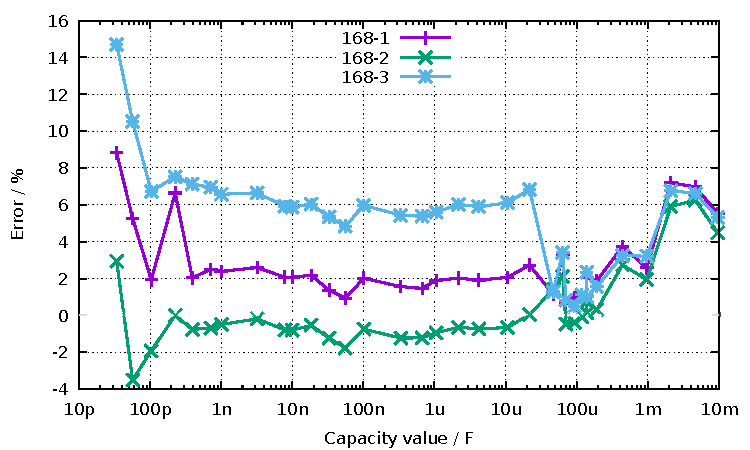
\includegraphics[width=1.\textwidth]{../GNU/Mega168all.pdf}
    \caption{three ATmega168}
    \label{fig:mega168all}
  \end{subfigure}
  ~
  \begin{subfigure}[b]{.5\textwidth}
    \centering
    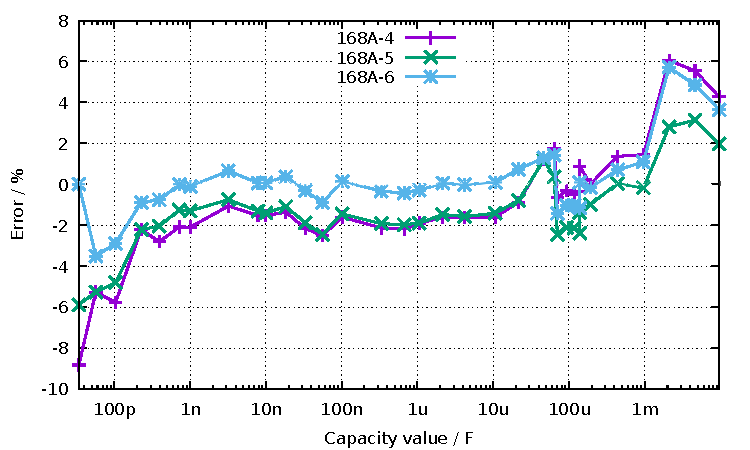
\includegraphics[width=1.\textwidth]{../GNU/Mega168Aall.pdf}
    \caption{three ATmega168A}
    \label{fig:mega168Aall}
  \end{subfigure}
\caption{capacity measurement error, not calibrated}
\end{figure}

\begin{figure}[H]
\centering
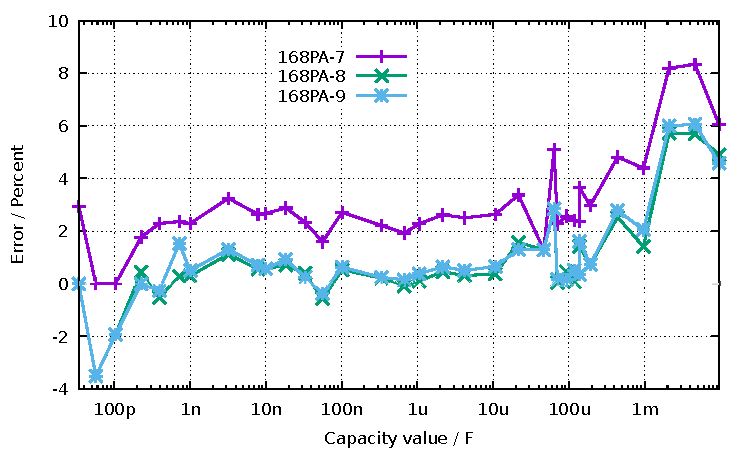
\includegraphics[width=.93\textwidth]{../GNU/Mega168PAall.pdf}
\caption{capacity measurement error of three ATmega168PA, not calibrated}
\label{fig:mega168PAall}
\end{figure}

\begin{figure}[H]
  \begin{subfigure}[b]{.5\textwidth}
    \centering
    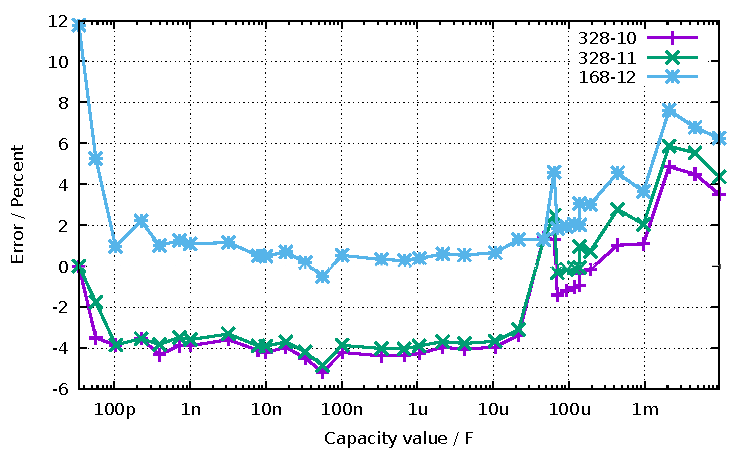
\includegraphics[width=1.\textwidth]{../GNU/Mega328all.pdf}
    \caption{three ATmega328}
    \label{fig:mega328all}
  \end{subfigure}
  ~
  \begin{subfigure}[b]{.5\textwidth}
    \centering
    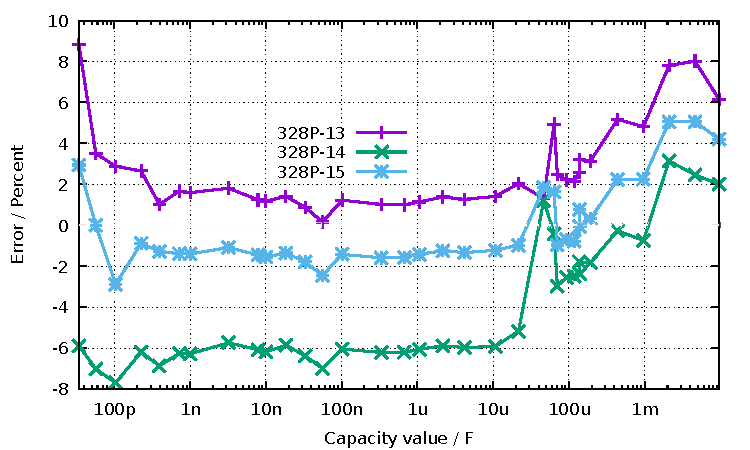
\includegraphics[width=1.\textwidth]{../GNU/Mega328Pall.pdf}
    \caption{three ATmega328P}
    \label{fig:mega328Pall}
  \end{subfigure}
\caption{capacity measurement error, not calibrated}
\end{figure}

To get the best accuracy you must adapt the software to the individual characteristic of your ATmega exemplar.
For this you can set a correction voltage REF\_C\_KORR for the comparator, which will be used for measurement of little capacity values.
A correction of \(1mV\) will reduce the measurement results to 0.11\% .
For big capacity values you can specify with the per mill value C\_H\_KORR, how much your capacity values are measured too big.
Because the capacitors with big values are most electrolytic capacitors with worse quality factor, the measurement of
the capacity value is difficult. So it is also extra difficult to get the difference to the real value of a capacitor.

Especially with the ATmega168 processors I have noticed a anomaly of measurement results of little capacity values,
which depend on the slew rate of the voltage during loading of the capacitor.
Figure~\ref{fig:mega168optcap} shows the error of the capacity measurement when only the zero value is respected
(168-3-A), with correction factor for little capacitors REF\_C\_KORR=66 as well as the correction factor for big
capacitors C\_H\_KORR=5 (168-3-B), plus additional as gradient 168-3-C  with a model of the slew rate dependency of little capacitor 
measurements (COMP\_SLEW1=4000 und COMP\_SLEW2=220). Also the self-discharge of big capacitors is respected with gradient 168-3-C.
The component with the slew rate dependent value is computed with \(\frac{COMP\_SLEW1}{cval+COMP\_SLEW2} - \frac{COMP\_SLEW1}{COMP\_SLEW2}\),
where cval is the measured capacity value with pF units.

\begin{figure}[H]
\centering
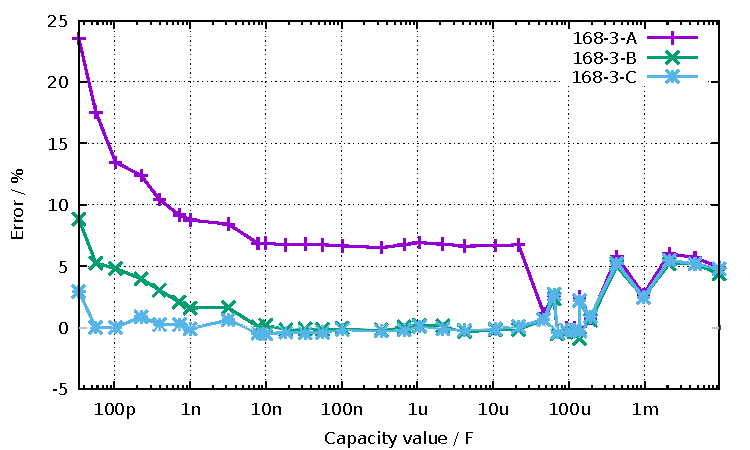
\includegraphics[width=.93\textwidth]{../GNU/Mega168cap_opt.pdf}
\caption{Improvement of the capacitor measurement of one ATmega168}
\label{fig:mega168optcap}
\end{figure}

\subsection{Automatic calibration of the capacitor measurement}

The automatic calibration is build in two parts. The first part find out the zero offset of the capacity measurement.
For that the mean value of the capacity measured without connected capacitor is build. 
A mean value for all 6 measurement combinations is build with 8 repetitions.
After successfull determination the zero offsets are written to the EEprom and will be used for further measurements.
More difficult was the clearance of the variance of the different ATmega processors for little capacitors (\textless \(40 \mu F\)),
which is shown in Figure~\ref{fig:mega168all}, \ref{fig:mega168Aall} and \ref{fig:mega168PAall}.
As a significant reason for this is found the different characteristic (Offset voltage) of the analog comparator.

The date of measurement of nine different processors is shown in figure~\ref{fig:CompAdjust} .
The ''diff2ref'' points show the difference of the voltage of a loaded capacitor of \(660nF\) to the
individual internal reference voltages (band gap).
Ideally this difference Voltage should be zero, if the analog comparator has stopped the loading by the signal to
the processor. The short handling time of the processor should not result to a measurably rising of the 
capacitor voltage of this relative big capacitor.
The ''CapErr'' points show the estimated measurement errors of each processor out of figure~\ref{fig:mega168all}, \ref{fig:mega168Aall} 
and \ref{fig:mega168PAall} with per mill units.
It is noticeable, how the ''CapErr'' points will follow the ''diff2ref'' points.
Therefore the ''diff'' points show the difference between the particular ''CapErr'' and ''diff2ref'' points.
With a mean value of the ''diff'' points we can get a good estimation for the correction of the capacitor
measurements together with the difference voltage of the loaded capacitor and the internal reference.

For the second part of adjustment you must connect a capacitor to pin~1 and pin~3. This capacitor should have
a good quality factor and should have a capacity between \(100nF\) and \(20\mu F\).
It should be a film capacitor, as far as possible not a ceramic capacitor und in no case a electrolytic capacitor.
You don't need to know the exact value of this capacitor.

\begin{figure}[H]
\centering
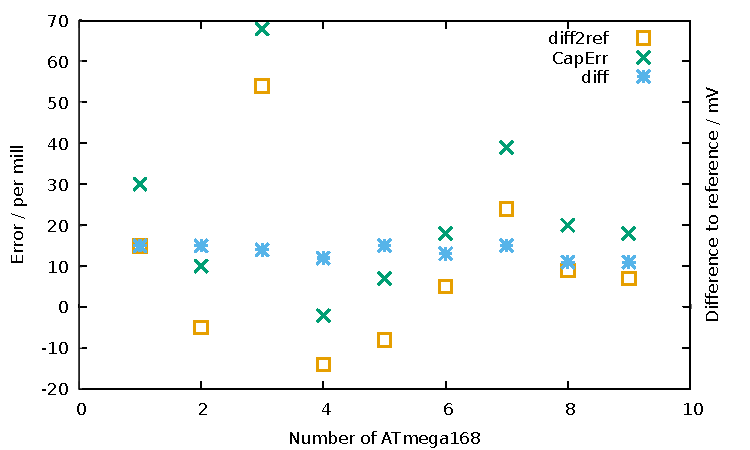
\includegraphics[width=.8\textwidth]{../GNU/ComparatorAdjust.pdf}
\caption{Date of nine ATmega168 processors}
\label{fig:CompAdjust}
\end{figure}

The figures~\ref{fig:mega168cal}, \ref{fig:mega168Acal}, \ref{fig:mega168PAcal}, \ref{fig:mega328cal} and \ref{fig:mega328Pcal}
 shows the measurement results
of the different processors with a standard software after the auto calibration.
The flash of the processors was loaded with the same software, only the Makefile  option ''PARTNO = '' must be
adapted to the different processor type (''m168'', ''m168p'', ''m328'' or ''m328p'') for the avrdude program.
After loading the data the selftest was started for each ATmega and a capacitor with \(330nF\) was connected
during test No.~10 to pin~1 and pin~3.

\begin{figure}[H]
  \begin{subfigure}[b]{.5\textwidth}
    \centering
    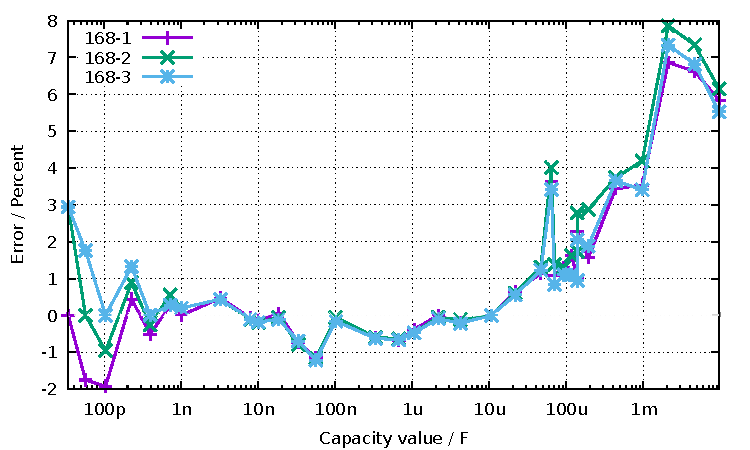
\includegraphics[width=1.\textwidth]{../GNU/Mega168cal.pdf}
    \caption{three ATmega168}
    \label{fig:mega168cal}
  \end{subfigure}
  ~
  \begin{subfigure}[b]{.5\textwidth}
    \centering
    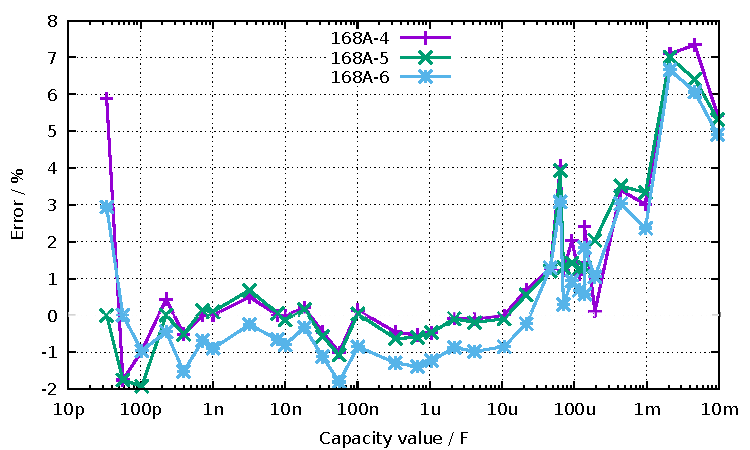
\includegraphics[width=1.\textwidth]{../GNU/Mega168Acal.pdf}
    \caption{three ATmega168A}
    \label{fig:mega168Acal}
  \end{subfigure}
  \caption{capacity measurement error, calibrated}
\end{figure}

\begin{figure}[H]
\centering
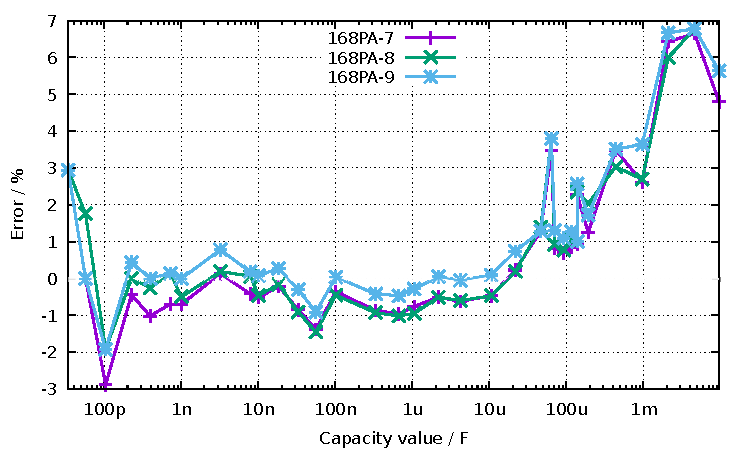
\includegraphics[width=.93\textwidth]{../GNU/Mega168PAcal.pdf}
\caption{capacity measurement error of three ATmega168PA, calibrated}
\label{fig:mega168PAcal}
\end{figure}

\begin{figure}[H]
  \begin{subfigure}[b]{.5\textwidth}
    \centering
    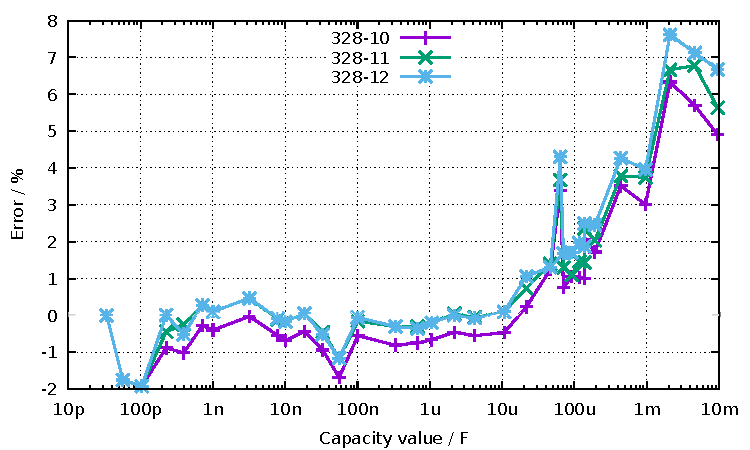
\includegraphics[width=1.\textwidth]{../GNU/Mega328cal.pdf}
    \caption{three ATmega328}
    \label{fig:mega328cal}
  \end{subfigure}
  ~
  \begin{subfigure}[b]{.5\textwidth}
    \centering
    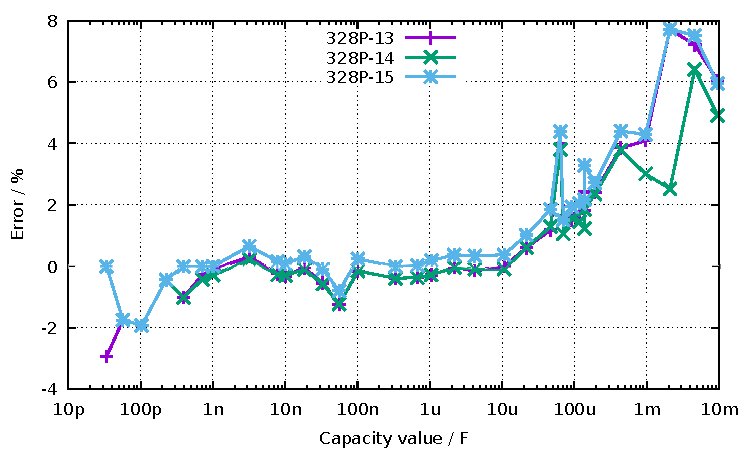
\includegraphics[width=1.\textwidth]{../GNU/Mega328Pcal.pdf}
    \caption{three ATmega328P}
    \label{fig:mega328Pcal}
  \end{subfigure}
  \caption{capacity measurement error, calibrated}
\end{figure}

At last I will make more clear the effect of the AUTO\_CAL option in the selftest program.
The following figure~\ref{fig:MegaAuto} shows the results from the three ATmega processors
with the biggest error of measurement, one measurement before the calibration and another
measurement after the calibration.
The points marked with the ending ''unc'' shows the the errors without calibration.
The lines with the ending ''cal'' shows the error results of the \textbf {same processors} 
with the \textbf {same software} after the calibration in the selftest section.
The reason for the measurement errors for big capacitors \textgreater(\(40\mu F\)) is
not yet known. All used capacitors for this series of measurements are film capacitors or
ceramic capacitors (\(56pF\), \(100pF\) and \(3.3nF\)), no electrolytical capacitors are used.

\begin{figure}[H]
\centering
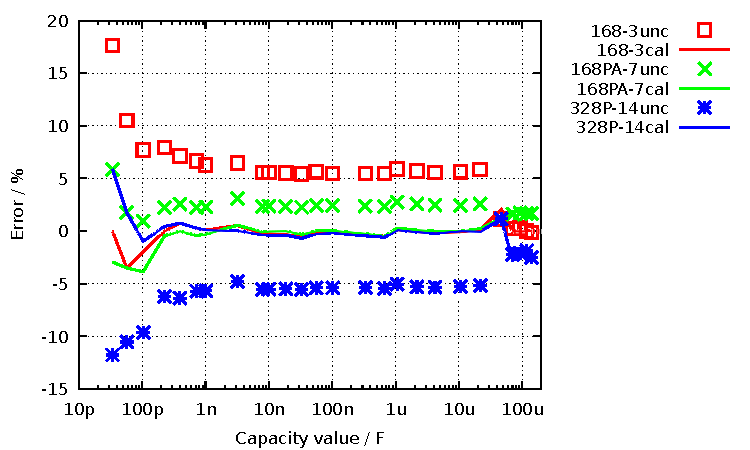
\includegraphics[width=.93\textwidth]{../GNU/MegaAuto.pdf}
\caption{Error of capacitor measurement of three ATmega, before and after the calibration}
\label{fig:MegaAuto}
\end{figure}

The circuit with a ATmega644 or ATmega1284 provides a capacitor for calibration at the printed board.
The figure \ref{fig:Mega1284} shows the results of the capicitor measurements with a ATmega1284,
with the on board \(100nF\) ceramic capacitor as well as with a external \(220nF\) foil capacitor, compared
to the results of a ATmega328 on another printed board.

\begin{figure}[H]
\centering
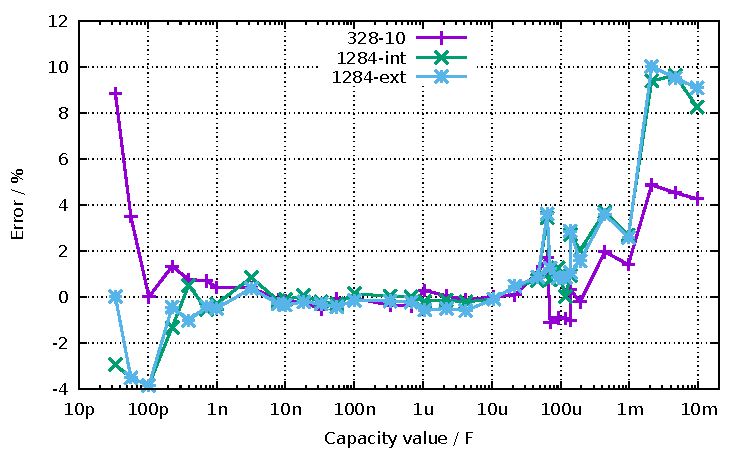
\includegraphics[width=.93\textwidth]{../GNU/Mega1284.pdf}
\caption{Error of capacitor measurements with a ATmega1284 compared to the ATmega328 results}
\label{fig:Mega1284}
\end{figure}

